\fancychapter{EMYS: the \emph{Sueca} player}
\label{chapter:approach}

Revising the purposes of this work, presented in Section~\ref{sec:goals}, the robotic agent that plays \emph{Sueca} has two main tasks: to choose an adequate card to play and to interact socially according to the game state.
In order to achieve these goals, some state-of-the-art approaches have been reviewed and considered for the implementation in our domain.
Thus the current chapter aims to carefully describe the decisions that were taken, some limitations imposed by the domain, as well as enhancements that have been made.
It starts with an overview of the whole system, proceeds with the implementation of the artificial player and last of all, details the development of the social agent.

\section{Architecture Overview}
\label{section:architecture_overview}

The model presented in Figure~\ref{fig:model} organises all the components involved in this system and their communications.
It considers a scenario where an embodied agent plays a physical card game against human players over a touch table.

\begin{figure}[ht]
  \centering
    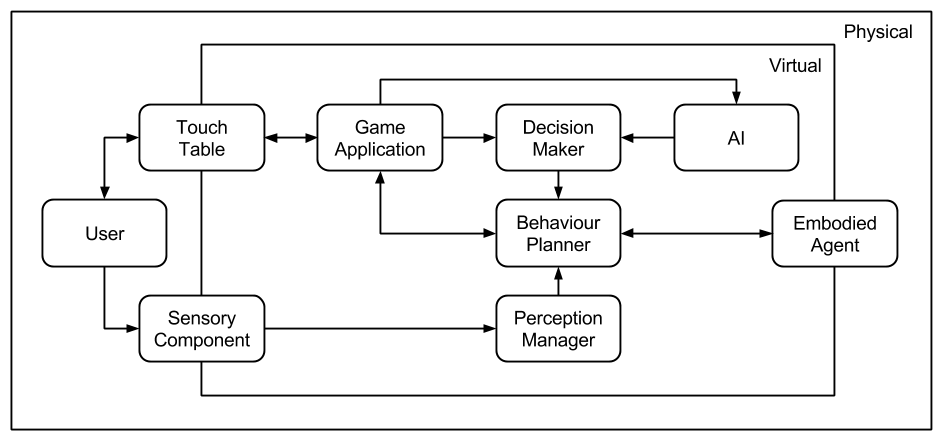
\includegraphics[width=1\textwidth]{./img/architecture}
  \caption{System architecture using components}
\label{fig:architecture}
\end{figure}

First of all, this model distinguishes physical components from virtual ones.
However, some entities are presented as both physical and virtual components and will not be detailed since their usage in this system did not demand any extensions for the scope of our domain (\emph{Touch Table}, \emph{Sensory Component} and \emph{Embodied Agent}).

The basic work-flow that illustrates the main functionalities of each component is as follows.
The human players, \emph{Users}, play with physical cards on top of a \emph{Touch Table}, and their game actions are managed by the \emph{Game Application} and communicated to both the \emph{\ac{ai}} and the \emph{Decision Maker}.
%\todo{check the sensory components!}
Besides their game actions, \emph{Users} also produce another sort of events that are captured by the \emph{Sensory Component} and handled by the \emph{Perception Manager}, for instance, face movements or the source direction of spoken interactions.
The \emph{\ac{ai}} includes all the reasoning about the game and decides the next move of the artificial player.
However, the \emph{Embodied Agent} will not only play a certain card, but will also include social behaviours.
As a result, the \emph{Decision Maker} balances the \emph{\ac{ai}} decisions and game information to produce an appropriate sequence of behaviours and inform them to \emph{Behaviour Planner}.
Lastly, the \emph{Behaviour Planner}, after receiving high-level intention-directed instructions, builds a suitable plan to execute the chosen instructions, considering the state of the \emph{Embodied Agent}, information from \emph{Perception Manager}, and additional game information from the \emph{Game Application}.

\begin{figure}[ht]
  \centering
    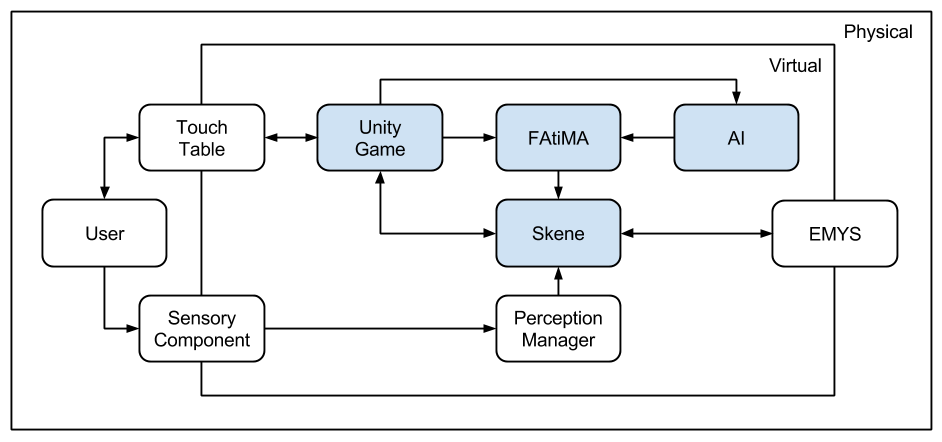
\includegraphics[width=1\textwidth]{./img/model}
  \caption{System architecture using modules}
\label{fig:model}
\end{figure}

%\todo{confirmar com o Tiago se sai uma seta do skene para o unity!!!}
The previously described architecture is instantiated as shown in Figure~\ref{fig:model} and the blue modules are thalamus communicating entities.
This concept arises from the Thalamus Framework \cite{Ribeiro}, which enables the usage of entities that can be registered at runtime in a server in order to send and receive specific messages.
These entities are publishers and subscribers of the channels they want to write on and listen to, respectively.
The implementation provided by this framework works by simply inherit from the \emph{ThalamusClient} class and implement the interfaces of the messages that the entity wants to exchange.

The \emph{Unity Game} module is responsible for displaying the interface of the game, reading the physical cards, publishing all the relevant game events and subscribing to the plays of artificial players.

The chosen \emph{Behaviour Planner} is \emph{Skene} \cite{Ribeiroa}, which tightens the communication between the world and an embodied agent with a high-level behaviour description language, also known as utterances.
These utterances might include instructions for gazing, pointing, animating or sound, among other things.
Additionally, considering some instructions require target positions or other game information, Skene subscribes to \emph{Unity game} messages to keep that information updated.

The \emph{\ac{ai}} and \emph{FAtiMA} modules answer to our primary goals, for that reason, their implementations are carefully detailed in Section~\ref{sec:artificial_player} and Section~\ref{sec:behaviour_planner}, respectively.

\section{An intelligent player}%The artificial player}
\label{sec:artificial_player}

This section will describe the most relevant implementation details of the artificial player.
After thoroughly analysing state-of-the-art techniques to solve imperfect information games, and considering \emph{Sueca} is, at this moment, computationally unsolved, the chosen approach was \ac{pimc}.
To implement this search technique, there are three key concepts or algorithms that require a full understanding: the Information Set, the PICM Search and the MinMax Algorithm.

\subsection*{Information Set}

An information set represents all the visible information during a game, and also inferred information based on certain events.
The player must keep an instance of the information set per game and update it when necessary.
It stores the known hand of the player and a deck with all the cards whose owner is unknown.
As result, each time another player plays a card, it should be removed from that deck.

The purpose of managing unplayed cards is to sample possible card distributions for the other three players with their real conditions.
These sampled distributions will be used during the \ac{pimc} search and the closer they are to the real world, the better the search returning value will be.
Additionally, the information set keeps track of suits per player and, when a player does not follow the leadsuit of a trick, it removes that suit from the player possible suits.
By possessing this information, sampling the distributions gets closer to the world, however it increased the complexity of the sampling process.
The method builds a \ac{csp} where:
\begin{itemize}
\item variables are the unplayed cards;
\item each domain is the set of players that still have that suit;
\item and the constraints are the number of times a player can be assigned to a card.
\end{itemize}


\subsection*{\ac{pimc} Search}

The following pseudo-code of the \ac{pimc} search algorithm guided the implementation.
To recapitulate the main point of this algorithm, considering it can choose up to \#Moves($I$), it samples $N$ possible card distributions for the other three players and calculates the reward of playing each possible move for the $N$ sampled worlds. The returned move is the one that gave more accumulated reward.

\begin{algorithm}
	\caption{PIMC search algorithm}
	\begin{algorithmic}[1]
		\Procedure{PIMC}{InfoSet $I$, int $N$}
			\ForAll {$m \in$ Moves($I$)}
				\State $val[m]$ = 0
			\EndFor
			\ForAll {$i \in \{ 1..N\}$}
				\State $x$ = Sample($I$)
				\ForAll {$m \in$ Moves($I$)}
					\State $val[m]$ += PerfInfoValue($x$, $m$)
				\EndFor
			\EndFor
			\State \textbf{return} $\underset{m}{argmax}\{ val[m] \}$
		\EndProcedure
	\end{algorithmic}
\end{algorithm}


\subsection*{MinMax Algorithm}

Bla bla bla


\subsection{Drawbacks}

Bla bla bla


\subsection{Enhancements}

Bla bla bla

\section{A cooperative and non-cooperative player}%Behaviour Planner Component}
\label{sec:behaviour_planner}

Robot has been implemented...


\clearpage

